\section{TÍNH ĐƠN ĐIỆU VÀ CỰC TRỊ CỦA HÀM SỐ}
\subsection{LÝ THUYẾT CẦN NHỚ}
\subsubsection{Tính đơn điệu của hàm số}
\begin{enumerate}[\iconMT]
	\item \indam{Định nghĩa:} Cho hàm số $y=f(x)$ xác định trên $K$ ($K$ là khoảng, đoạn hoặc nửa khoảng). \\
\begin{minipage}[b]{6cm}
\begin{khung4}{Ghi nhớ 1}
	Hàm số đồng biến trên $K$ nếu
	$\forall x_1,\,x_2 \in K$, $$ x_1<x_2 \Rightarrow f(x_1)<f(x_2)$$
	\centerline{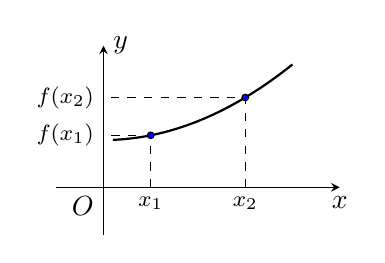
\begin{tikzpicture}[>=stealth,scale=0.6]
		\draw[->] (-1,0)--(0,0)%
		node[below left]{$O$}--(5,0) node[below]{$x$};
		\draw[->] (0,-1) --(0,3) node[right]{$y$};
		\draw [black,thick, domain=0.2:4, samples=100] %
		plot (\x, {0.1*(\x)^2+1});
		\draw [dashed] (1,0)node[below]{\footnotesize$x_1$} --(1,1.1)--(0,1.1)node[left]{\footnotesize$f(x_1)$};
		\draw [dashed] (3,0)node[below]{\footnotesize$x_2$} --(3,1.9)--(0,1.9)node[left]{\footnotesize$f(x_2)$};
		\draw[fill=blue] (1,1.1) circle(2pt);
		\draw[fill=blue] (3,1.9) circle(2pt);
	\end{tikzpicture}}\\
Trên $K$, đồ thị là một "\textbf{đường đi lên}" khi xét từ trái sang phải.
\end{khung4}
\end{minipage}\hspace{0.5cm}
\begin{minipage}[b]{6cm}
\begin{khung4}{Ghi nhớ 2}
		Hàm số nghịch biến trên $K$ nếu
		$\forall x_1,\,x_2 \in K$, $$ x_1<x_2 \Rightarrow f(x_1)>f(x_2)$$
		\centerline{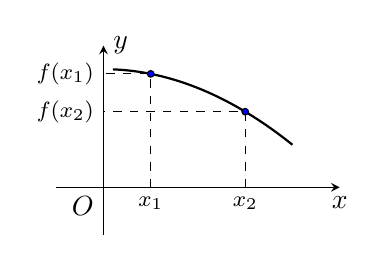
\begin{tikzpicture}[>=stealth,scale=0.6]
			\draw[->] (-1,0)--(0,0)%
			node[below left]{$O$}--(5,0) node[below]{$x$};
			\draw[->] (0,-1) --(0,3) node[right]{$y$};
			\draw [thick, domain=0.2:4, samples=100] %
			plot (\x, {-0.1*(\x)^2+2.5});
			\draw [dashed] (1,0)node[below]{\footnotesize$x_1$} --(1,2.4)--(0,2.4)node[left]{\footnotesize$f(x_1)$};
			\draw [dashed] (3,0)node[below]{\footnotesize$x_2$} --(3,1.6)--(0,1.6)node[left]{\footnotesize$f(x_2)$};
			\draw[fill=blue] (1,2.4) circle(2pt);
			\draw[fill=blue] (3,1.6) circle(2pt);
		\end{tikzpicture}}\\
	Trên $K$, đồ thị là một "\textbf{đường đi xuống}" khi xét từ trái sang phải.
\end{khung4}
\end{minipage}
	\item \indam{Liên hệ giữa đạo hàm và tính đơn điệu:}
	Cho hàm số $y=f(x)$ có đạo hàm trên khoảng $(a;b)$.
	\begin{boxdn}
	\begin{listEX}[1]
		\item [$\bullet$] Nếu $y'\ge 0$, $\forall x \in (a;b)$ và dấu bằng chỉ xảy ra tại hữu hạn điểm thì hàm số $y=f(x)$ đồng biến trên $(a;b)$.
		\item [$\bullet$] Nếu $y'\le 0$, $\forall x \in (a;b)$ và dấu bằng chỉ xảy ra tại hữu hạn điểm thì hàm số  $y=f(x)$ nghịch biến trên $(a;b)$.
	\end{listEX}
	\end{boxdn}
\end{enumerate}
\subsubsection{Cực trị của hàm số}
\begin{enumerate}[\iconMT]
	\item \indam{Định nghĩa:} Cho hàm số $y=f(x)$ xác định và liên tục trên khoảng $(a ; b)$ ( $a$ có thể là $-\infty, b$ có thể là $+\infty)$ và điểm $x_0 \in(a ; b)$.
	\begin{boxdn}
	\begin{itemize}
		\item [$\bullet$] Nếu tồn tại số $h>0$ sao cho $f(x)<f\left(x_0\right)$ với mọi $x \in\left(x_0-h ; x_0+h\right) \subset(a ; b)$ và $x \neq x_0$ thì ta nói hàm số $f(x)$ đạt cực đại tại $x_0$.
		\item [$\bullet$] Nếu tồn tại số $h>0$ sao cho $f(x)>f\left(x_0\right)$ với mọi $x \in\left(x_0-h ; x_0+h\right) \subset(a ; b)$ và $x \neq x_0$ thì ta nói hàm số $f(x)$ đạt cực tiểu tại $x_0$.
	\end{itemize}
	\end{boxdn}
	\item \indam{Định lý:} Giả sử hàm số $y=f(x)$ liên tục trên khoảng $(a ; b)$ chứa điểm $x_0$ và có đạo hàm trên các khoảng $\left(a ; x_0\right)$ và $\left(x_0 ; b\right)$. Khi đó:
	\begin{boxdn}
	\begin{itemize}
		\item [$\bullet$] Nếu $f^{\prime}(x)<0$ với mọi $x \in\left(a ; x_0\right)$ và $f^{\prime}(x)>0$ với mọi $x \in\left(x_0 ; b\right)$ thì $x_0$ là một điểm cực tiểu của hàm số $f(x)$.
		\item [$\bullet$] Nếu $f^{\prime}(x)>0$ với mọi $x \in\left(a ; x_0\right)$ và $f^{\prime}(x)<0$ với mọi $x \in\left(x_0 ; b\right)$ thì $x_0$ là một điểm cực đại của hàm số $f(x)$.
	\end{itemize}
	\end{boxdn}
	\item \indam{Các tên gọi:}\\
		\begin{tikzpicture}[smooth,samples=300,scale=1.15,>=stealth]
			\draw[->,>=stealth] (-2.5,0)--(2.7,0) node[below]{$x$};
			\draw[->,>=stealth] (0,-1.5)--(0,4) node[right]{$y$};
			\draw (0,0) node[above left]{$O$};
			\draw[blue,domain=-2:2,line width = 1.2pt] plot(\x,{(\x)^3-3*(\x)+1})node[right]{$y=f(x)$};
			\draw[fill=black] (1,0) circle(1pt) (1,-1) circle(2pt) (0,-1) circle(1pt) (-1,0) circle(1pt) (-1,3) circle(2pt) (0,3) circle(1pt);
			\draw[dashed] (1,0)node[above]{\small$x_2$}--(1,-1)--(0,-1)node[left]{\small$y_2$} (-1,0)node[below]{\small$x_1$}--(-1,3)--(0,3)node[right]{\small$y_1$};
			
			\draw[-,dotted] (-0.5,3.7)--(4,3.7)node[right]{$(x_1;y_1)$ là điểm cực đại của đồ thị hàm số;}; 
			\draw[->,dotted] (-0.5,3.7)--(-1,3.15);
			\node[right] at (4.5,3.1) {$\bullet$ $x_1$ là điểm cực đại của hàm số;};
			\node[right] at (4.5,2.5) {$\bullet$ $y_1$ là giá trị cực đại của hàm số.};
			
			\draw[-,dotted] (2,-1)--(2,1)--(4,1)node[right]{$(x_2;y_2)$ là điểm cực tiểu của đồ thị hàm số;}; \draw[->,dotted] (2,-1)--(1.15,-1);
			\node[right] at (4.5,0.4) {$\bullet$ $x_2$ là điểm cực tiểu của hàm số;};
			\node[right] at (4.5,-0.2) {$\bullet$ $y_2$ là giá trị cực tiểu của hàm số.};
		\end{tikzpicture}
\end{enumerate}
\subsection{PHÂN LOẠI VÀ PHƯƠNG PHÁP GIẢI TOÁN}
\begin{dang}{Bài toán tìm khoảng đơn điệu và cực trị của hàm số cho trước}
	\begin{listEX}[1]
		\item [\ding{172}] Tìm tập xác định $\mathscr{D}$ của hàm số $y=f(x)$ .
		\item [\ding{173}] Tính đạo hàm $f'(x)$. Tìm các điểm $x_i \,(i = 1, 2, ..., n)$ thuộc $\mathscr{D}$ mà tại đó đạo hàm bằng $0$ hoặc không xác định.
		\item [\ding{174}] Sắp xếp các điểm $x_i$ theo thứ tự tăng dần, xét dấu $y'$ và lập bảng biến thiên. Từ đây, nêu các khoảng đồng biến, nghịch biến và các điểm cực trị.
	\end{listEX}
\end{dang}
\indamm{Ghi nhớ cách xét dấu:}
\begin{note}
\begin{enumerate}[\iconCH]
		% \item Nếu $$f'(x)=(x-a)(x-b)^2(x-c)^{2n}(x-d)^{2n+1},\,\forall n \in \mathbb{N}*$$
		% thì phương trình $f'(x)=0$ có
		% \begin{itemize}
		% 	\item 	$x=a$ là nghiệm đơn;
		% 	\item  $x=b$ là nghiệm kép;
		% 	\item  $x=c$ là nghiệm bội chẵn;
		% 	\item  $x=d$ là nghiệm bội lẻ.
		% \end{itemize}
		\item Khi xét dấu $f'(x)$ thì $f'(x)$ sẽ không đổi dấu khi qua nghiệm kép (nghiệm bội chẵn) và đổi dấu khi qua nghiệm đơn (nghiệm bội lẻ).
	\end{enumerate}
	% \begin{tikzpicture}[smooth,samples=300,scale=0.8,>=stealth,font=\footnotesize]
	% 	\draw[->] (-3.5,0)--(6,0) node[below]{$x$};
	% 	\draw[->] (0,-1.5)--(0,4) node[left]{$y$};
	% 	\draw (0,0) node[above left]{$O$};
	% 	\draw[blue,line width=0.7pt,domain=-2.15:1.5] plot(\x,{(\x+2)*(\x-1)^2});
	% 	\draw[blue,line width=0.7pt,domain=1.5:4.7] plot(\x,{-1*(\x-1.64)*(\x-4)^2})node[below]{$y=f'(x)$};
	% 	\draw[fill=red] (-2,0)node[above left]{$x_1$} circle(1.5pt) (1,0)node[below]{$x_2$} circle(1.5pt) (4,0)node[above right]{$x_4$} circle(1.5pt) (1.64,0)node[above right]{$x_3$} circle(1.5pt);
	% 	\draw[dashed,<-] (-1.8,-0.2)--(0.5,-2.3)node[below]{\fbox{\scriptsize\text{Nghiệm bội lẻ}}};
	% 	\draw[dashed,->](0.5,-2.3)--(1.58,-0.2);
	% 	\draw[dashed,<-] (1,0.2)--(2,3)node[above]{\fbox{\scriptsize\text{Nghiệm bội chẵn}}};
	% 	\draw[dashed,->](2,3)--(3.9,0.1);
	% 	\end{tikzpicture}
\end{note}
\boxmini{BÀI TẬP TỰ LUẬN}

\begin{vd}
	Tìm các khoảng đơn điệu và các điểm cực trị của hàm số sau
	\begin{tasks}(3)
		\task $ y=-x^3+3x^2-4$;
		\task $ y=x^3-3x^2+1$;
		\task $y=x^3+3x^2+3x+2$;
		\task $y=-2x^4+4x^2$;
		\task $y=x^4+4x^3-1$;
		\task $y=-16x^4+x-1$.
	\end{tasks}
	\loigiai{
	\begin{enumEX}[a)]{1}
		\item Tập xác định: $\mathscr{D}=\mathbb{R}$. \\
		Đạo hàm: $y'=-3x^2+6x$.\\
		Xét $y'=0 \Leftrightarrow -3x^2+6x=0 \Leftrightarrow
		\hoac{
			& x=0 \\
			& x=2 }$
		Bảng biến thiên:\begin{center}
			
\begin{tikzpicture}
				\tkzTabInit[nocadre=false,lgt=0.7,espcl=2.1,deltacl=0.6]
				{$x$ /0.6,$y'$ /0.6,$y$ /2}
				{$-\infty$,$0$,$2$,$+\infty$}
				\tkzTabLine{,-,$0$,+,$0$,-,}
				\tkzTabVar{+/$+\infty$, -/$-4$,+/$0$,-/$-\infty$}
			\end{tikzpicture}
		\end{center}
		\item Ta có: $ y'=3x^2-6x\Rightarrow y'=0\Leftrightarrow \hoac{&x=0\\&x=2.} $\\
		Từ bảng biến thiên suy ra hàm số đồng biến trên khoảng $ (-\infty;0) $ và $ (2;+\infty). $
		\begin{center}
			
\begin{tikzpicture}
				\tkzTabInit[nocadre=false,lgt=1,espcl=3]
				{$x$ /1,$y'$ /1,$y$ /2}
				{$-\infty$,$0$, $2$,$+\infty$}
				\tkzTabLine{,+,$0$,-,$0$,+, }
				\tkzTabVar{-/ $-\infty$,+/$1 $ ,-/$-3$,+/$+\infty$}
			\end{tikzpicture}
		\end{center}
		\item Hàm số đã cho xác định trên $\mathscr{D}=\mathbb{R}$.\\
		Ta có $y'=3x^2+6x+3$. Cho $y'=0 \Leftrightarrow 3x^2+6x+3=0 \Leftrightarrow x=-1$.\\
		Bảng biến thiên
		\begin{center}
			
\begin{tikzpicture}
				\tkzTabInit[lgt=1,espcl=3]
				{$x$/0.7,$y'$/0.7,$y$/2}
				{$-\infty$,$-1$,$+\infty$}
				\tkzTabLine{,+,0,+,}
				\tkzTabVar{-/$-\infty$,R/,+/$+\infty$}
				
			\end{tikzpicture}
		\end{center}
		Vậy hàm số đồng biến trên $\mathbb{R}$.
		\item Tập xác định của hàm số là $ \mathscr{D}=\mathbb{R}$.\\
		Ta có $y'=-8x^3+8x$.
		Cho $y'=0 \Leftrightarrow -8x^3+8x=0 \Leftrightarrow 8x(-x^2+1)=0$\\
		\centerline{$ \Leftrightarrow \left[\begin{aligned}
				&8x=0 \\
				&-x^2+1=0
			\end{aligned}\right. \Leftrightarrow \left[\begin{aligned}
				&x=0 \\
				&x^2=1
			\end{aligned}\right. \Leftrightarrow \left[\begin{aligned}
				&x=0 \\
				&x=\pm 1.
			\end{aligned}\right. $}
		Bảng biến thiên
		\begin{center}
			
\begin{tikzpicture}
				\tkzTabInit[lgt=1,espcl=3]
				{$x$/0.7,$y'$/0.7,$y$/2}
				{$-\infty$,$-1$,$0$,$1$,$+\infty$}
				\tkzTabLine{,+,0,-,0,+,0,-,}
				\tkzTabVar{-/$-\infty$,+/ $2$/,-/$0$,+/$2$,-/$-\infty$}
			\end{tikzpicture}
		\end{center}
		Vậy hàm số đồng biến trên mỗi khoảng $(-\infty;-1)$ và $(0;1)$,\\
		\indent{ } hàm số nghịch biến trên mỗi khoảng $(-1;0)$ và $(1;+\infty)$.
		\item Hàm số đã cho xác định trên $\mathscr{D}=\mathbb{R}$.\\
		Ta có $y'=4x^3+12x^2=0=4x^2(x+3)$.\\
		Cho $y'=0 \Leftrightarrow 4x^2(x+3)=0 \Leftrightarrow \left[\begin{aligned}
			&x=0 \\
			&x=-3.
		\end{aligned}\right.$\\
		Bảng biến thiên
		\begin{center}
			
\begin{tikzpicture}
				\tkzTabInit[lgt=1,espcl=3]
				{$x$/0.7,$y'$/0.7,$y$/2}
				{$-\infty$,$-3$,$0$,$+\infty$}
				\tkzTabLine{,-,0,+,0,+,}
				\tkzTabVar{+/$+\infty$,-/$-28$ /,R,+/$+\infty$}
			\end{tikzpicture}
		\end{center}
		Vậy hàm số nghịch biến trên khoảng $(-\infty;-3)$ và đồng biến trên khoảng $(-3;+\infty)$.
		\item Ta có $y'=-64x^3+1<0\Leftrightarrow x>\dfrac{1}{4}$ nên hàm số nghịch biến trên khoảng $\left(\dfrac{1}{4};+\infty\right)$.
\end{enumEX}}
\end{vd}

\begin{vd}
	Tìm các khoảng đơn điệu và cực trị của các hàm số sau:
	\begin{tasks}(3)
		\task $y=\dfrac{2x+1}{x+1}$;
		\task $y=\dfrac{3x+1}{x-1}$;
		\task $y=\dfrac{x^2+2x+2}{x+1}$;
		\task $y=x+\dfrac{4}{x}$;
		\task $y=\sqrt{x^2-2x}$;
		\task $y=x-3\sqrt[3]{x^2}$ .
	\end{tasks}
	\loigiai{
		\begin{enumEX}[a)]{1}
			\item Ta có $y'=\dfrac{1}{(x+1)^2} > 0, \forall x \in \mathbb{R} \backslash \{-1\}$.\\
			Vậy hàm số đồng biến trên $(-\infty ;-1)$ và $(-1 ;+\infty)$.\\
			Hàm số không có cực trị.
			\item Ta có $y'=\dfrac{-4}{(x-1)^2}>0,\,\forall x\in\mathbb{R}\setminus\{1\}$.\\
			Do vậy hàm số nghịch biến trên các khoảng  $(-\infty;1)$; $(1;+\infty)$.\\
			Hàm số không có cực trị.
			\item \begin{itemize}
				\item TXĐ: $\mathscr{D}=\mathbb{R}\setminus \left\{-1\right\}$.
				\item $y'=\dfrac{x^2+2x}{(x+1)^2}$, $y'=0\Leftrightarrow \hoac{& x=-2 \\ & x=0.}$\\
				Ta có bảng biến thiên
				\begin{center}
					\begin{center}
						
\begin{tikzpicture}
							\tkzTabInit[nocadre=True,lgt=1,espcl=2]
							{$x$ /0.7,$y'$ /0.7,$y$ /2}
							{$-\infty$,$-2$,$-1$,$0$,$+\infty$}
							\tkzTabLine{,+,$0$,-,d,-,$0$,+,}
							\tkzTabVar{-/$-\infty$,+/$-2$,-D+/$-\infty$/$+\infty$,-/$2$,+/$+\infty$}
						\end{tikzpicture}
					\end{center}
				\end{center}
				Hàm số đồng biến trên khoảng $\left( -\infty;-2\right)$ và $\left( 0;+\infty\right)$;  nghịch biến trên $(-2;-1)$ và $(-1;0)$.\\
				Hàm số đạt cực đại tại $x=-2$, giá trị cực đại $y=-2$\\
				Hàm số đạt cực tiểu tại $x=0$, giá trị cực tiểu $y=2$.\\
			\end{itemize}
			\item Tập xác định $\mathscr{D}=\mathbb{R}\setminus\{0\}$.\\
			Ta có $y'=1-\dfrac{4}{x^2}=\dfrac{x^2-4}{x^2}$, $y'=0\Leftrightarrow x=\pm 2$.\\
			Bảng biến thiên
			\begin{center}
				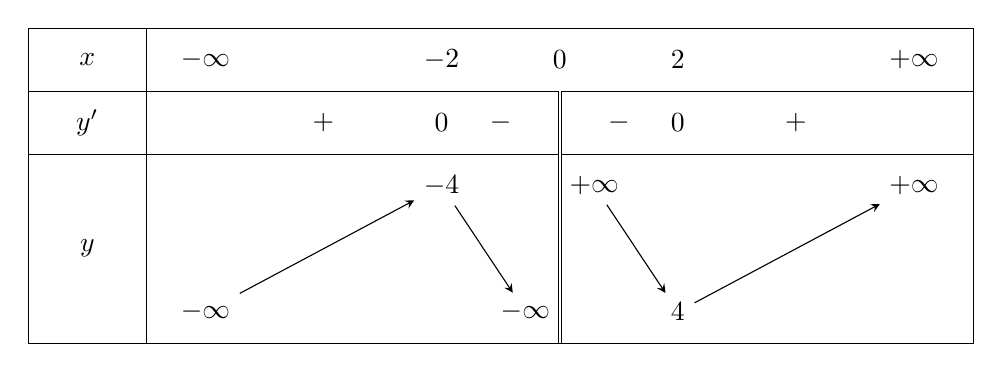
\begin{tikzpicture}[yscale=.8,xscale=1.5,]
					\begin{scope}[shift={(-.5,.5)}]
						\draw
						(0,0) rectangle +(8,-5)
						(0,-1)--+(0:8) (0,-2)--+(0:8) (1,0)--+(-90:5);
					\end{scope}
					\path
					(0,0) node{$x$}          % <<< dòng 1
					++(0:1) node{$-\infty$}
					++(0:2) node{$-2$}
					++(0:1) node{$0$}
					++(0:1) node{$2$}
					++(0:2) node{$+\infty$}
					(0,-1)   node{$y'$}         % <<< dòng 2
					++(0:2) node{$+$}
					++(0:1) node{$0$}
					++(0:.5) node{$-$}
					++(0:1) node{$-$}
					++(0:.5) node{$0$}
					++(0:1) node{$+$}
					(0,-3)   node{$y$}       % <<< dòng 3
					++(0:1) ++(-90:1)  node (A) {$-\infty$}
					++(0:2) ++(90:2) node (B) {$-4$}
					++(0:1) ++(-90:2) node (C)[left]
					{$-\infty$}
					++(90:2) node (D)[right]{$+\infty$}
					++(0:1) ++(-90:2) node (E) {$4$}
					++(0:2) ++(90:2) node (F) {$+\infty$};
					\draw[-stealth] (A)--(B);
					\draw[-stealth] (B)--(C);
					\draw[-stealth] (D)--(E);
					\draw[-stealth] (E)--(F);
					\draw[double] (4,-.5)--(4,-4.5);
				\end{tikzpicture}
			\end{center}
			Hàm số đồng biến trên khoảng $\left( -\infty;-4\right)$ và $\left( 2;+\infty\right)$; nghịch biến trên các khoảng $(-2;0)$ và $(0;2)$.\\
			Hàm số đạt cực đại tại $x=-2$, giá trị cực đại $y=-4$\\
			Hàm số đạt cực tiểu tại $x=2$, giá trị cực tiểu $y=4$\\
			\item Tập xác định: $\mathscr{D}=(-\infty;0]\cup [2;+\infty)$.\\
			Ta có $y'=\dfrac{x-1}{\sqrt{x^2-2x}},\forall x\in (-\infty;0)\cup (2;+\infty)$.\\
			$y'=0 \Leftrightarrow \dfrac{x-1}{\sqrt{x^2-2x}}=0 \Rightarrow x-1=0 \Leftrightarrow x=1 \notin \mathscr{D}$.\\
			Bảng biến thiên:
			\begin{center}
				
\begin{tikzpicture}
					\tkzTabInit[lgt=1,espcl=3]
					{$x$/0.7,$y'$/0.7,$y$/2}
					{$-\infty$,$0$,$2$,$+\infty$}
					\tkzTabLine{,-,d,h,d,+,}
					\tkzTabVar{+/$+\infty$,-H/$0$/,-/$0$,+/$+\infty$}
				\end{tikzpicture}
			\end{center}
			Vậy hàm số nghịch biến trên khoảng $(-\infty;0)$ và đồng biến trên khoảng $(2;+\infty)$.\\
			Hàm số không có cực trị.
			\item Tập xác định: $\mathscr{D}=\mathbb{R}$.\\
			Đạo hàm $y'=1-\dfrac{2}{\sqrt[3]{x}}$, xác định với mọi $x\neq 0$.\\
			$y'=0\Leftrightarrow \sqrt[3]{x}=2\Leftrightarrow x=8$.\\
			Đạo hàm không xác định tại $x=0$.\\
			Bảng biến thiên
			\begin{center}
				
\begin{tikzpicture}
					\tkzTabInit[nocadre,lgt=1,espcl=2]{$x$/0.7,$y'$/0.7,$y$/2}{$-\infty$,$0$,$8$,$+\infty$}%
					\tkzTabLine{,+,d,-,z,+,}
					\tkzTabVar{-/$-\infty$ , +/$0$,-/$-4$, +/$+\infty$}%
				\end{tikzpicture}
			\end{center}
	\end{enumEX}}
\end{vd}

\begin{vd}
	Thể tích $V$ (đơn vị: centimét khối) của $1 \mathrm{~kg}$ nước tại nhiệt độ $T\,\left(0^{\circ} \mathrm{C} \leq T \leq 30^{\circ} \mathrm{C}\right)$ được tính bởi công thức	$$	V(T)=999,87-0,06426 T+0,0085043 T^2-0,0000679 T^3$$
	 Hỏi thể tích $V(T), \,0^{\circ} \mathrm{C} \leq T \leq 30^{\circ} \mathrm{C}$, giảm trong khoảng nhiệt độ nào?
	\loigiai{
		Xét hàm số  $V(T)=999{,}87-0{,}06426T+0{,}0085043T^2-0{,}0000679T^3$, với $T\in [0;30]$.\\
	Ta có $V'(T)=-0{,}0002037T^2+0{,}0170086T-0{,}06426$.\\
	$V'(T)=0\Leftrightarrow T=3{,}966514624=T_1$ hoặc $T=79{,}53176716\not\in [0;30]$.\\
	Bảng biến thiên của hàm số $V(T)$ như sau
	\begin{center}
		
\begin{tikzpicture}[font=\footnotesize,thick,>=stealth]
			\tikzset{double style/.append style={double distance=1.5pt}}
			\tkzTabInit[nocadre=false,lgt=1.2,espcl=2.5,deltacl=0.6,lw=.75pt,color,colorL=green!50,colorV=green!50]
			{$T$ /0.7, $V'(T)$ /0.8, $V(T)$ /2}
			{$0$,$T_1$,$30$}
			\tkzTabLine{ ,-,$0$,+, }
			\tkzTabVar{+/$V(0)$,-/$V(T_1)$,+/$V(30)$}
		\end{tikzpicture}
	\end{center}
	Từ bảng biến thiên suy ra, thể tích $V(T), 0^{\circ}\mathrm{C}\leq T \leq 30^{\circ}\mathrm{C}$, giảm trong khoảng nhiệt độ từ $0^\circ$C đến $3{,}966514624^\circ$C.}
\end{vd}

\boxmini{BÀI TẬP TRẮC NGHIỆM}
\ind{PHẦN I.} \inden{Câu trắc nghiệm nhiều phương án lựa chọn. Mỗi câu hỏi học sinh chỉ chọn một phương án.}\\
\setcounter{ex}{0}
\Opensolutionfile{ans}[ans/2D1-B1-d1-1]

\begin{ex}%[KSCL, Sở GD \& ĐT Hà Nam, 2018]%[Lê Quốc Hiệp, dự án 12EX10-18]%[2D1B1-2]%
	\immini
	{Cho hàm số $y=f(x)$ có đồ thị như hình vẽ bên. Hàm số $y=f(x)$ nghịch biến trên khoảng nào dưới đây?
		\haicot
		{$(\sqrt{2};+\infty)$}
		{$(-2;2)$}
		{$(-\infty;0)$}
		{\True $(0;\sqrt{2})$}
	}
	{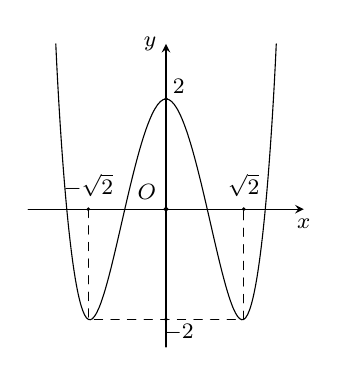
\begin{tikzpicture}[line cap=round,line join=round,x=1.0cm,y=1.0cm,>=stealth,scale=0.7]
			\draw[->,color=black,smooth,samples=100] (-2.5,0.) -- (2.5,0.) node[below] {\footnotesize $x$};
			\draw[->,color=black,smooth,samples=100] (0.,-2.5) -- (0.,3) node[left] {\footnotesize $y$};
			\draw plot[smooth,tension=.7] coordinates {(-2,3) (-1.41,-2)  (0,2) (1.41,-2) (2,3)};
			\draw[fill=black] (0,0) circle [radius=1pt] node[above left] {\footnotesize $O$};
			\fill (-1.41,0) node[shift={(90:2ex)}]{\footnotesize $-\sqrt{2}$} circle(1pt);
			\fill (1.41,0) node[shift={(90:2ex)}]{\footnotesize $\sqrt{2}$} circle(1pt);
			\fill (0,-2) node[shift={(-45:1.5ex)}]{\footnotesize $-2$} circle(1pt);
			\fill (0,2) node[shift={(45:1.5ex)}]{\footnotesize $2$} circle(1pt);
			\draw[dashed] (-1.41,0)|-(0,-2)-|(1.41,0);
	\end{tikzpicture}}
	\loigiai
	{
		Dựa vào đồ thị, ta thấy trên khoảng $(0;\sqrt{2})$ đồ thị đi xuống nên hàm số $y=f(x)$ nghịch biến trên khoảng đó.
	}
\end{ex}

\begin{ex}
	\immini{Cho hàm số $y=f(x)$ có đồ thị như hình vẽ bên. Mệnh đề nào sau đây là mệnh đề \textbf{sai}?
		\choice
		{Hàm số đạt cực đại tại $x=0$}
		{Hàm số có giá trị cực tiểu bằng $-2$}
		{\True Hàm số đồng biến trên $(-\infty; 2)$}
		{Hàm số nghịch biến trên $(0; 2)$}
	}
	{
		
		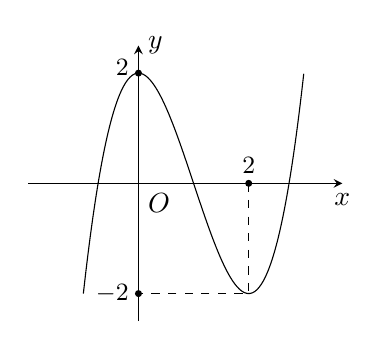
\begin{tikzpicture}[smooth,samples=300,scale=0.7,>=stealth]
			\draw[->] (-2,0)--(3.7,0) node[below]{$x$};
			\draw[->] (0,-2.5)--(0,2.5) node[right]{$y$};
			\draw (0,0) node[below right]{$O$};
			\draw[smooth,samples=100,domain=-1:3]
			plot(\x,{(\x)^3-3*(\x)^2+2});
			\draw[fill=black] (2,0) circle(1.5pt) (0,2) circle(1.5pt) (0,-2) circle(1.5pt);
			\draw[dashed] (2,0)node[above]{\small$2$}--(2,-2)--(0,-2)node[left]{\small$-2$} (0,2.1)node[left]{\small$2$};
		\end{tikzpicture}
	}
	
	\loigiai{
	}
	
\end{ex}

\begin{ex}
	\immini{
		Hàm số $y=f(x)$ có đồ thị là đường cong trong hình vẽ bên. Hàm số $y=f(x)$ đạt cực tiểu tại điểm nào dưới đây?
		\haicot
		{$x=2$}
		{\True $x=0$}
		{$x=-2$}
		{$x=4$}
	}{
		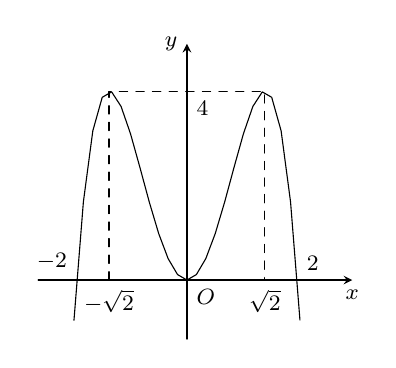
\begin{tikzpicture}[xscale=.7,yscale=.6, font=\footnotesize, line join=round, line cap=round, >=stealth]
			\draw[->] (-2.7,0)--(3,0) node[below]{$x$};
			\draw[->] (0,-1.25)--(0,5) node[left]{$y$};
			\draw[dashed] (-2^.5,0)--(-2^.5,4)--(2^.5,4)--(2^.5,0);
			\draw[domain=-2.05:2.05] plot(\x,{-(\x)^2*((\x)^2-4)});
			\path
			(0,0) node[below right]{$O$}
			(2,0) node[above right]{$2$}
			(-2,0) node[above left]{$-2$}
			(0,4) node[below right]{$4$}
			(-2^.5,0) node[below]{$-\sqrt{2}$}
			(2^.5,0) node[below]{$\sqrt{2}$};
		\end{tikzpicture}
	}
	\loigiai{
		Dựa vào đồ thị hàm số ta thấy hàm số đạt cực tiểu tại $x=0$.}
\end{ex}

\begin{ex}
	\immini{Cho hàm số $y=f(x)$ có bảng biến thiên như hình bên. Mệnh đề nào sau đây là mệnh đề đúng?
	\choice
	{Hàm số đồng biến trên khoảng $(-\infty;3)$}
	{Hàm số nghịch biến trên khoảng $(-2;+\infty)$}
	{Hàm số đạt cực đại tại $x=3$}
	{\True Hàm số đạt cực tiểu tại $x=2$}}{
	\begin{tikzpicture}
	\tkzTabInit[lgt=1.2,espcl=1.8,nocadre=True]
	{$x$/0.6,$f'(x)$/0.6,$f(x)$/2}{$-\infty$,$-2$,$2$,$+\infty$}
	\tkzTabLine{,+,0,-,0,+,}
	\tkzTabVar{-/$-\infty$,+/$3$,-/$0$,+/$+\infty$}
\end{tikzpicture}}
	\loigiai{
	}
	
\end{ex}

\begin{ex}
	Cho hàm số $y=f(x)$ có bảng biến thiên bên dưới
	\begin{center}
		\begin{tikzpicture}
			\tikzset{double style/.append style = {draw=\tkzTabDefaultWritingColor,double=\tkzTabDefaultBackgroundColor,double distance=2pt}}
			\tkzTabInit[lgt=1.2,espcl=2,nocadre=True]
			{$x$ /.7, $f’(x)$ /.7,$f(x)$ /2}
			{$-\infty$ , $-2$, $0$ ,$2$ ,$+\infty$}
			\tkzTabLine{ ,+,$0$,-,d,-,$0$,+, }
			\tkzTabVar{ -/ $-\infty$,+/ $-4$/,-D+/$- \infty$ /$+\infty$,-/ $4$,+ /$+\infty$}
		\end{tikzpicture}
	\end{center}
Khẳng định nào sau đây là khẳng định \textbf{sai}?
	\choice
	{Hàm số có hai điểm cực trị}
	{Tọa độ điểm cực đại của đồ thị hàm số là $(-2;-4)$}
	{\True Hàm số nghịch biến trên khoảng $(-2;2)$}
	{Hàm số đồng biến trên khoảng $(3;+\infty)$}
	\loigiai{
	}
\end{ex}


\begin{ex}
	Cho hàm số $y= - \dfrac{1}{3} x^3 - x -3 $. Mệnh đề nào dưới đây đúng?
	\choice
	{Hàm số đồng biến trên $(-\infty; 1)$ và trên $(1; +\infty)$}
	{\True Hàm số nghịch biến trên $\mathbb{R}$}
	{Hàm số đồng biến trên $(-1;1)$}
	{Hàm số đồng biến trên $\mathbb{R}$}
	\loigiai{
		Tập xác định $\mathscr D = \mathbb{R}$.\\
		$y'=-x^2 -1<0 $ với mọi $x$.\\
		Suy ra  hàm số đã cho nghịch biến trên $\mathbb{R}$.}
\end{ex} 


\begin{ex}
	Gọi $x_1$ là điểm cực đại $x_2$ là điểm cực tiểu của hàm số $y=-x^3+3x+2$. Tính $x_1+2x_2$.
	\choice{$2$}
	{$1$}
	{\True $-1$}
	{$0$}
	\loigiai{
		Ta có $y'=-3x^2+3$, $y'=0\Leftrightarrow x=\pm 1$.\\
		Vì $y'$ đổi dấu từ âm sang dương khi qua $x=-1$ và đổi dấu từ dương sang âm khi qua $x=1$ nên $x_2=-1$ là điểm cực tiểu và $x_1=1$ là điểm cực đại của hàm số. Do đó $x_1+2x_2=1-2=-1$.
	}
\end{ex} 


\begin{ex}
	Khoảng cách giữa hai điểm cực trị của đồ thị hàm số $y=x^3-3x^2+4$ bằng
	\choice
	{\True $2\sqrt{5}$}
	{$2\sqrt{2}$}
	{$2$}
	{$ 4 $}
	\loigiai{
		Ta có $y'=3x^2-6x$, $ y'=0\Rightarrow \hoac{&x=0\Rightarrow y=4\\&x=2\Rightarrow y=0.} $\\
		Suy ra hai điểm cực trị của đồ thị hàm số là $A(0;4),B(2;0)$.\\
		Do đó $AB=\sqrt{2^2+(-4)^2}=2\sqrt{5}$.
	}
\end{ex} 

\begin{ex}%[2D1B1]
	Hàm số $y=x^4-2x^2+1$ đồng biến trên khoảng nào dưới đây?
	\choice
	{\True $(-1;0)$}
	{$(-1;+ \infty)$}
	{$(-3;8)$}
	{$(- \infty ; -1)$}
	\loigiai
	{
		$y'= 4x^3-4x$ $\Rightarrow y'=0 \Leftrightarrow 4x^3-4x=0$ $\Leftrightarrow \hoac{x&= -1 \\ x&=0 \\ x &= 1}$\\
		Bảng xét dấu
		\begin{center}
			
\begin{tikzpicture}
				\tkzTabInit[nocadre=false, lgt=1, espcl=2.5]{$x$ /1,$y$ /1}{$-\infty$,$-1$,$0$,$1$,$+\infty$}
				\tkzTabLine{,-,$0$,+,$0$,-,$0$,+}
			\end{tikzpicture}
		\end{center}
	}
	
\end{ex} 

\begin{ex}%[2HK1-13-ChuyenLeQuyDon-QuangTri]%[2D1B2-1]%
	Cho hàm số $ y = - \dfrac{1}{4}x^4 + \dfrac{1}{2}x^2 - 3 $. Khẳng định nào sau đây là khẳng định đúng?
	\choice
	{Hàm số đạt cực tiểu tại $ x = -3 $}
	{ \True Hàm số đạt cực tiểu tại $ x = 0 $}
	{Hàm số đạt cực đại tại $ x = 0 $}
	{Hàm số đạt cực tiểu tại $ x = -1 $}
	\loigiai{
		Ta có $ y' = - x^3 + x = - x (x^2 - 1) $.
		Ta có bảng biến thiên như hình bên
		\begin{center}
			
\begin{tikzpicture}[scale=1]
				\tkzTabInit[lgt=1.5,espcl=2.5]{$x$  /1,$y'$  /1,$y$ /2}
				{$-\infty$,$ -1 $,$ 0 $,$ 1 $,$+\infty$}%
				\tkzTabLine{,+,z,-,z,+,z,-,}
				\tkzTabVar{-/$ -\infty $,+/   $\dfrac{-11}{4}$ /,-/ $-3$,+/$ \dfrac{-11}{4} $,-/$ -\infty $}
				%\tkzTabIma{1}{3}{2}{$ 0 $}
			\end{tikzpicture}
		\end{center}
	}
\end{ex} 

\begin{ex}
	Cho hàm số $y=\dfrac{3x-1}{x-2}$. Mệnh đề nào dưới đây là đúng?
	\choice
	{Hàm số nghịch biến trên $\mathbb{R}$}
	{Hàm số đồng biến trên các khoảng $(-\infty;2)$ và $(2;+\infty)$}
	{\True Hàm số nghịch biến trên các khoảng $(-\infty;2)$ và $(2;+\infty)$}
	{Hàm số đồng biến trên $\mathbb{R}\setminus\{2\}$}
	\loigiai{Tập xác định là $\mathscr{D}=\mathbb{R}\setminus\{2\}$.\\
		Có $y'=\dfrac{-5}{(x-2)^2}<0$, $\forall x\in\mathscr{D}$ nên hàm số nghịch biến trên các khoảng $(-\infty;2)$ và $(2;+\infty)$.}
	
\end{ex} 

\begin{ex}
	Cho hàm số $y=\dfrac{x-2}{x+3}$. Mệnh đề nào dưới đây đúng?
	\choice
	{Hàm số nghịch biến trên khoảng $(-\infty;-3)\cup (-3;+\infty) $}
	{\True Hàm số đồng biến trên khoảng $(-\infty;-3) $ và $(-3;+\infty)$}
	{Hàm số nghịch biến trên khoảng $(-\infty;-3)$ và $(-3;+\infty)$}
	{Hàm số đồng biến trên khoảng $(-\infty;-3)\cup (-3;+\infty) $}
	\loigiai{
		Tập xác định $\mathscr{D}=\mathbb{R}\setminus \{-3\}$. Ta có $y'=\dfrac{5}{(x+3)^2}>0$, $\forall x\in\mathscr{D}$.\\ Suy ra hàm số đồng biến trên khoảng $(-\infty;-3)$ và $(-3;+\infty)$.
	}
\end{ex} 

\begin{ex}
	Gọi $y_{\text{CĐ}},\,y_{\text{CT}}$ lần lượt là giá trị cực đại và giá trị cực tiểu của hàm số $y=\dfrac{x^2+3x+3}{x+2}$. Giá trị của biểu thức $y_{\text{CĐ}}^2-2y_{\text{CT}}^2$ bằng
	\choice
	{$8$}
	{\True $7$}
	{$9$}
	{$6$}
	\loigiai{
		Ta có $y'=\dfrac{x^2+4x+3}{(x+2)^2}$; $y'=0 \Leftrightarrow \left[\begin{aligned}
			&x=-1 \\
			&x=-3
		\end{aligned}\right. $. \\
		Bảng biến thiên
		\begin{center}
			
\begin{tikzpicture}
				\tkzTab
				[lgt=1,espcl=2] % tùy chọn
				{$x$/0.7, $y'$/0.7, $y$/2} % cột đầu tiên
				{$-\infty$, $-3$, $-2$, $-1$, $+\infty$} % hàng 1 cột 2
				{,+,0,-,d,-,0,+,} % hàng 2 cột 2
				{-/ $-\infty$, +/ $-3$, -D+/ $-\infty$ / $+\infty$, -/ $1$, +/ $+\infty$} % hàng 3 cột 2
			\end{tikzpicture}
		\end{center}
		Từ bảng biến thiên ta tìm được $y_{\text{CĐ}}=-3;\,y_{\text{CT}}=1$ $ \Rightarrow $ $y_{\text{CĐ}}^2-2y_{\text{CT}}^2$ $=9-2=7$.}
\end{ex} 

\begin{ex}
	Tìm điểm cực tiểu của hàm số $f(x)=(x-3)\mathrm{e}^x$.
	\choice
	{$x=3$}
	{$x=0$}
	{\True $x=2$}
	{$x=1$}
	\loigiai{
		\begin{itemize}
			\item Ta có $f'(x)=\mathrm{e}^x(x-2)$, $f''(x)=\mathrm{e}^x(x-1)$.
			\item $f'(x)=0\Rightarrow x=2$ và $f''(2)=\mathrm{e}^2>0$.
		\end{itemize}
		Vậy hàm số đã cho đạt cực tiểu tại $x=2$.}
\end{ex} 

\begin{ex}
	Cho hàm số $y=x^2+4\ln(3-x)$. Tìm giá trị cực đai $y_\text{CĐ}$ của hàm số đã cho.
	\choice
	{$y_\text{CĐ}=2$}
	{\True $y_\text{CĐ}=4$}
	{$y_\text{CĐ}=1+4\ln2$}
	{$y_\text{CĐ}=1$}
	\loigiai{
		Tập xác định $\mathscr{D}=(-\infty;3)$.\\
		Đạo hàm $y'=2x-\dfrac{4}{3-x}=\dfrac{-2x^2+6x-4}{3-x}$.\\
		$y'=0\Leftrightarrow -2x^2+6x-4=0\Leftrightarrow \hoac{&x=1\\&x=2}$.\\
		Bảng biến thiên
		\begin{center}
			
\begin{tikzpicture}[>=stealth]
				\tkzTabInit[nocadre=false,lgt=1,espcl=2,deltacl=0.5]{$x$/.7,$y'$/.7,$y$/2}
				{$-\infty$,$1$,$2$,$3$}
				\tkzTabLine{,-,0,+,0,-,d}
				\tkzTabVar{+/$+\infty$,-/$1+4\ln 2$,+/$4$,-D/$-\infty$}
			\end{tikzpicture}
		\end{center}
		Hàm số đạt cực đại tại $x=2$, $y_\text{CĐ}=4$.
	}
\end{ex} 


\begin{ex}%[2D1K2]
	Cho hàm số $y = f(x)$ xác định trên $\mathbb{R}$ và có đạo hàm $y' = f'(x) = 3x^3 - 3x^2$. Mệnh đề nào sau đây \textbf{sai}?
	\choice
	{Trên khoảng $(1;+\infty)$ hàm số đồng biến}
	{Trên khoảng $(-1;1)$ hàm số nghịch biến}
	{\True Đồ thị hàm số có hai điểm cực trị}
	{Đồ thị hàm số có một điểm cực tiểu}
	\loigiai
	{
		Ta có: $y' = 0 \Leftrightarrow 3x^3 - 3x^2 = 0 \Leftrightarrow \hoac{& x = 0 \\& x = 1.}$\\
		Bảng biến thiên:
		\begin{center}
			
\begin{tikzpicture}[>=stealth]
				\tkzTabInit[nocadre, lgt=1, espcl=2.5]
				{$x$ /0.7,$y'$ /0.7,$y$ /1.7}
				{$-\infty$,$0$,$1$,$+\infty$}
				\tkzTabLine{,-,$0$,-,$0$,+,}
				\tkzTabVar{+/ $+\infty$, R, -/{\text{CT}}, +/ $+\infty$}
			\end{tikzpicture}
		\end{center}
		Hàm số đồng biến trên khoảng $(1;+\infty)$.\\
		Hàm số nghịch biến trên khoảng $(-\infty;1)$.\\
		Hàm số đạt cực tiểu tại $x = 1$.
	}
\end{ex} 

\begin{ex}%[2D1B2]
	Cho hàm số $ y=f(x) $ liên tục trên $ \mathbb{R} $ và có đạo hàm $ f'(x)=x(x-1)^2(x-2)^3 $. Số điểm cực trị của hàm số $ y=f(x) $ là
	\choice{1}{\True 2}{0}{3}
	\loigiai{	Ta có bảng xét dấu của $ f'(x) $:
		\begin{center}
			\begin{tikzpicture}
				\tkzTabInit[lgt=2,espcl=1.5]%
				{$x$ /1,$f'(x)$ /1}
				{$-\infty$ , $0$ , $1$ , $2$ ,$+\infty$}
				\tkzTabLine{ ,+,0,-,0,-,0,+,}
			\end{tikzpicture}
		\end{center}
		Dựa vào bảng xét dấu ta thấy $ f(x) $ có 2 điểm cực trị.
}\end{ex} 



\begin{ex}%[2D1K2-2]%
	\immini{Cho hàm số bậc bốn $ y=f(x) $. Biết $f'(x) $ có đồ thị như hình bên. Khẳng định nào sau đây là khẳng định đúng?
		\choice
		{Hàm số $f(x)$ đồng biến trên khoảng $(-\infty;0)$}
		{Hàm số $f(x)$ nghịch biến trên khoảng $(-1;1)$}
		{Hàm số $f(x)$ có đúng một điểm cực tiểu}
		{\True Hàm số $f(x)$ có đúng một điểm cực đại}
	}{
		\begin{tikzpicture}[>=stealth,line join=round,line cap=round,font=\footnotesize,scale=0.7,smooth]
			\draw[->] (-3,0)--(7,0)node[below]{$x$};
			\foreach \x in {-2,-1,1,2,3,4}\draw[shift={(\x,0)}] (0,2pt)--(0,-2pt) node[below]{\scriptsize $\x$};
			\draw[->] (0,-2)--(0,3)node[right]{$y$};
			\draw[] plot[smooth,tension=.65] coordinates{(-1.7,-2) (-1,0) (0,.7) (1,0)(2.7,-1.2)(4,0) (5,2.5)}node[right]{$y=f'(x)$};
		\end{tikzpicture}
	}
	\loigiai{
		\immini{Dựa vào đồ thị, ta có bảng biến thiên như hình vẽ. \\
		}{% Cần khai báo \usepackage{tkz-tab}
			
\begin{tikzpicture}[scale=.8, font=\footnotesize, line join=round, line cap=round, >=stealth]
				\tkzTabInit[nocadre=false,lgt=1,espcl=2,deltacl=0.5]{$x$/.7 ,$y'$/.7,$y$/2}
				{$-\infty$ , $-1$ , $1$, $ 4 $, $+\infty$}
				\tkzTabLine{ , - , $0$ ,+, $ 0 $, -, $0$ , + , }
				\tkzTabVar{+/$+\infty$ , -/$f(-1)$ ,+/$f(-1)$ ,-/$ f(4) $, +/$+\infty$}
		\end{tikzpicture}}
	}
\end{ex} 

\begin{ex}
	\immini{
		Cho hàm số $y=f(x)$ xác định và liên tục trên $\mathbb{R}$. Biết rằng hàm số $f(x)$ có đạo hàm $f'(x)$ và hàm số $y=f'(x)$ có đồ thị như hình vẽ. Khi đó nhận xét nào sau đây đúng?
		\choice
		{\True Hàm số $f(x)$ không có cực trị}
		{Đồ thị hàm số $f(x)$ có đúng $2$ điểm cực tiểu}
		{Đồ thị hàm số $f(x)$ có đúng một cực đại}
		{Hàm số $f(x)$ có $3$ cực trị}
	}{
		\begin{tikzpicture}[scale=.8,font=\footnotesize, line join=round,line cap=round,>=stealth]
			\draw[->] (-2.5,0)--(2.5,0)node[below]{$x$};
			\draw[->] (0,-1)--(0,3.5)node[left]{$y$};
			\draw[samples=100,domain=-1.7:1.7] plot(\x,{(\x)^4-2*(\x)^2+1});
			\draw[dashed] (-1,0)node[below]{$-1$}circle(1pt) (1,0)node[below]{$1$}circle(1pt) (0,1)node[above right]{$1$}circle(1pt);
		\end{tikzpicture}
	}
	\loigiai{
		Dựa vào đồ thị ta thấy $f'(x)\geq 0$, với mọi $x\in\mathbb{R}$.\\
		Suy ra, hàm số $f(x)$ không có cực trị.
	}
\end{ex} 


\Closesolutionfile{ans}

\ind{PHẦN II.} \inden{Câu trắc nghiệm đúng sai. Trong mỗi ý a), b), c), d) ở mỗi câu, học sinh chọn đúng hoặc sai.}\\
\Opensolutionfile{ans}[ans/2D1-B1-d1-2]

\begin{ex}
	Cho hàm số $y=f(x)$ liên tục trên $\mathbb{R}$ và có bảng xét dấu đạo hàm như hình bên.
	\begin{center}
		
\begin{tikzpicture}
			\tikzset{double style/.append style = {draw=\tkzTabDefaultWritingColor,double=\tkzTabDefaultBackgroundColor,double distance=2pt}}
			\tkzTabInit[nocadre=false, lgt=1, espcl=1.2]{$x$ /0.7,$y'$ /1}{$-\infty$,$0$,$1$,$2$,$+\infty$}
			\tkzTabLine{,+,$0$,-,d,+,$0$,+,}
		\end{tikzpicture}
	\end{center}
	% \immini{
		\choiceTF
		{Hàm số đồng biến trên khoảng $(-\infty;1)$}
		{\True Hàm số đồng biến trên khoảng $(1;+\infty)$}
		{Hàm số đạt cực đại tại $x=2$}
		{Hàm số có một điểm cực đại và hai điểm cực tiểu}
	% }{\vspace{0.1cm}
		%}
	\loigiai{
		Ta có bảng biến thiên như sau:
		\begin{center}
			
\begin{tikzpicture}
				\tikzset{double style/.append style = {draw=\tkzTabDefaultWritingColor,double=\tkzTabDefaultBackgroundColor,double distance=2pt}}
				\tkzTabInit[lgt=1.1,espcl=2,nocadre=True]
				{$x$ /.7, $y'$ /.7,$y$ /2}
				{$-\infty$ , $0$, $1$ ,$2$ ,$+\infty$}
				\tkzTabLine{ ,+,$0$,-,d,+,$0$,+, }
				\tkzTabVar{ -/,+/ /,-/,R,+/$+\infty$}
			\end{tikzpicture}
		\end{center}
	Từ đây, suy ra:
		\begin{enumerate}[a)]
			\item Hàm số đồng biến trên khoảng $(-\infty;1)$ là khẳng định sai.
			\item Hàm số đồng biến trên khoảng $(1;+\infty)$ là khẳng định đúng.
			\item Hàm số đạt cực đại tại $x=2$ là khẳng định sai.
			\item Hàm số có một điểm cực đại và hai điểm cực tiểu là khẳng định sai.
		\end{enumerate}
	}
	
\end{ex} 

\begin{ex}
	Cho hàm số $y=x^3-3x^2+4$ có đồ thị $(C)$. Gọi $A$, $B$ là hai điểm cực trị của $(C)$.
	\choiceTF
	{\True Tập xác định của hàm số là $\mathbb{R}$}
	{Hàm số đồng biến trên khoảng $(0;2)$}
	{\True PTĐT qua hai điểm cực trị của đồ thị hàm số là $2x+y-4=0$}
	{\True Diện tích của tam giác $OAB$ bằng $4$, với $O$ là gốc tọa độ}
	\loigiai{
		\begin{enumerate}[a)]
			\item Hàm số đa thức nên có tập xác định là $D=\mathbb{R}$.
			\item Ta có 
			\begin{itemize}
				\item [$\bullet$] $y'=3x^2-6x$ và $y'=0 \Leftrightarrow x=0$ hoặc $x=2$.
			\end{itemize}
			Bảng biến thiên:
			\begin{center}
				
\begin{tikzpicture}
					\tkzTabInit[lgt=1,espcl=3]
					{$x$ /0.7, $y'$ /0.7, $y$ /2.5}
					{$-\infty$,$0$,$2$,$+\infty$}
					\tkzTabLine{,+,$0$,-,$0$,+,}
					\tkzTabVar{-/$-\infty$,+/$4$,-/$0$,+/$+\infty$}
				\end{tikzpicture}
			\end{center}
		Suy ra hàm nghịch biến trên $(0;2)$.
			\item Tọa độ $A(0;4)$, $B(2;0)$. PTĐT $AB$ là
			$$\dfrac{x-0}{2-0}=\dfrac{y-4}{0-4} \Leftrightarrow 2x+y-4=0$$
			\item Diện tích tam giác vuông $OAB$ là $S_{OAB}=\dfrac{1}{2}OA \cdot OB=4$.
		\end{enumerate}

	}
\end{ex} 

\begin{ex}
	Cho hàm số $y=\dfrac{x^2+2x+2}{x+1}$ có đồ thị $(C)$. Gọi $A$, $B$ lần lượt là điểm cực tiểu và điểm cực đại của $(C)$.
	\choiceTF
	{Tập xác định của hàm số là $\mathbb{R}$}
	{Hàm số nghịch biến trên khoảng $(-2;0)$}
	{Tọa độ điểm $A(-2;-2)$, $B(0;2)$}
	{Khoảng cách giữa hai điểm cực trị là $AB=2\sqrt{5}$}
	\loigiai{
		\begin{enumerate}[a)]
			\item Đặt điều kiện mẫu số khác 0, ta được $x+1 \ne 0 \Leftrightarrow x \ne -1$. Suy ra $\mathscr{D}=\mathbb{R}\setminus \left\{-1\right\}$.
			\item $y'=\dfrac{x^2+2x}{(x+1)^2}\Rightarrow y'=0\Leftrightarrow \hoac{& x=-2 \\ & x=0.}$\\
			Ta có bảng xét dấu của hàm $f'(x)$ như sau
			\begin{center}
					
\begin{tikzpicture}
					\tkzTabInit[nocadre=false,lgt=1,espcl=3]
					{$x$ /0.7,$y'$ /0.7,$y$ /2}
					{$-\infty$,$-2$,$-1$,$0$,$+\infty$}
					\tkzTabLine{,+,$0$,-,d,-,$0$,+,}
					\tkzTabVar{-/$-\infty$,+/$-2$,-D+/$-\infty$/$+\infty$,-/$2$,+/$+\infty$}
				\end{tikzpicture}
			\end{center}
			Dựa vào bảng xét dấu ta thấy rằng hàm số $y=f'(x)$ nghịch biến trên $(-2;-1)$ và $(-1;0)$.
			\item Tọa độ điểm $A(0;2)$, $B(-2;-2)$
			\item Độ dài $AB=\sqrt{(-2-0)^2+(-2-2)^2}=2\sqrt{5}$.
		\end{enumerate}

	}
\end{ex} 


\begin{ex}
	Xét một chất điểm chuyển động dọc theo trục $Ox$. Toạ độ của chất điểm tại thời điểm $t$ được xác định bởi hàm số $x(t)=t^3-6t^2+9t$ với $t\geq 0$. Khi đó $x'(t)$ là vận tốc của chất điểm tại thời điểm $t$, kí hiệu $v(t)$; $v'(t)$ là gia tốc chuyển động của chất điểm tại thời điểm $t$, kí hiệu $a(t)$.
	\choiceTF
	{Phương trình hàm vận tốc là $v(t)=3t^2-6t+9$}
	{\True Phương trình hàm gia tốc là $a(t)=6t-12$}
	{Vận tốc của chất điểm tăng khi $t\in (0;1)$ hoặc  $t \in (3;+\infty)$}
	{Vận tốc của chất điểm giảm khi $t\in (1;3)$}
	\loigiai{
		\begin{enumerate}
			\item $v(t)=x'(t)=3t^2-12t+9$
			\item $a(t)=v'(t)=6t-12$.
			\item Xét $v'(t)=6t-12$, $v'(t)=0\Leftrightarrow t=2$\\
			Bảng xét dấu
			\begin{center}
				\begin{tikzpicture}
					\tkzTabInit[nocadre=false,lgt=2,espcl=2.1]
					{$t$ /0.6,$v'(t)$ /0.6}
					{$0$,$2$,$+\infty$}
					\tkzTabLine{,-,$0$,+,}
				\end{tikzpicture}
			\end{center}
			Suy ra vận tốc của chất điểm tăng khi $t\in (2;+\infty) $, giảm khi $t\in (0;2)$.
		\end{enumerate}
	}
\end{ex} 

\Closesolutionfile{ans}